\section{Beispiele für numerische Lösung nichtlinearer Gleichungssysteme}

\begin{example2}{Einleitendes Beispiel}
    $$f_1(x_1, x_2) = x_1^2 + x_2 - 11 = 0$$
    $$f_2(x_1, x_2) = x_1 + x_2^2 - 7 = 0$$
    Gesucht sind die Lösungen des Gleichungssystems. Diese lassen sich interpretieren als die Nullstellen der Funktion $\textbf{f}: \R^2 \to \R^2$ gemäss:
    $$\textbf{f}(x) = \begin{pmatrix} f_1 (x_1, x_2) \\ f_2 (x_1, x_2) \end{pmatrix} = \begin{pmatrix} x_1^2 + x_2 - 11 \\ x_1 + x_2^2 - 7 \end{pmatrix} = \begin{pmatrix} 0\\ 0 \end{pmatrix}$$
    Offensichtlich lässt sich ein solches System nicht in die Form $Ax = b$ bringen. 

    \begin{minipage}{0.5\linewidth}
    Geometrisch lassen sich die Lösungen als Schnittpunkte der beiden Funktionen interpretieren.\\
    Explizite Darstellung der Kurven:
    $$x_2 = 11 - x_1^2$$
    $$x_2 = \sqrt{7 - x_1}$$
    Schnittpunkte:
    $$\overline{\textbf{x}_1} = \begin{psmallmatrix} 3 \\ 2 \end{psmallmatrix}, \quad \overline{\textbf{x}_2} = \begin{psmallmatrix} -2.8 \\ 3.2 \end{psmallmatrix}$$
    $$\overline{\textbf{x}_3} = \begin{psmallmatrix} -3.8 \\ -3.3 \end{psmallmatrix}, \quad \overline{\textbf{x}_4} = \begin{psmallmatrix} 3.4 \\ -1.7 \end{psmallmatrix}$$
    \end{minipage}
    \begin{minipage}{0.5\linewidth}
    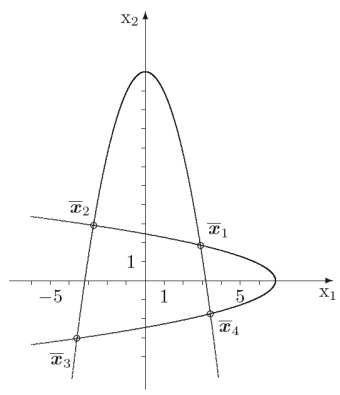
\includegraphics[width=\linewidth]{einleitendes_bsp_kap5.png}
    \end{minipage}
\end{example2}